\documentclass[12pt]{article}

\usepackage{tabularx}
\usepackage[table]{xcolor}
\usepackage{multirow}

\usepackage{amsmath, amssymb}
\usepackage{mathtools}

\usepackage{tikz}
\usetikzlibrary{positioning}
\usetikzlibrary{patterns}
\usetikzlibrary{matrix,backgrounds}
\usetikzlibrary{arrows,shapes,trees}
\usetikzlibrary{chains,shapes}
\usetikzlibrary{arrows}
\usetikzlibrary{decorations.pathmorphing}

\usepackage{pgfplots}
\tikzset{declare function={unitstep(\x)=notless(\x,0);}}
\tikzset{declare function={delta(\x)=equal(\x,0);}}


\usepackage[margin=1.1in,footskip=.25in]{geometry}


\usepackage[most]{tcolorbox}

\tcbset{
    frame code={}
    center title,
    left=10pt,
    right=10pt,
    top=10pt,
    bottom=10pt,
    colback=gray!5,
    colframe=gray,
    width=\dimexpr\textwidth\relax,
    enlarge left by=0mm,
    boxsep=5pt,
    arc=0pt,outer arc=0pt,
}

\renewcommand{\baselinestretch}{1.3} 

\begin{document}

\section{Signals \& Systems - Introduction}

Signal : Any time varying physical phenomenon that is intended to convey information is called as signal .
\newline \newline
\noindent
Signal is a function of time .


\noindent
e.g : human voice , voltage on telephone wires , electric signal , $\dots$
\newline \newline
\noindent
System : system is a device which operates on signals according to its characteristics .


\begin{center}
\begin{tikzpicture}
%\draw (3,1) rectangle (6,-1);
\draw node (a) at (1,0) {input};
%\draw node (b) at (4.5,0) {system};
\node[draw, inner sep=10mm] (b) at (4.5,0) {system};
\draw node (c) at (8,0) {output};
%\draw[->,->=latex,thick] (a) -- (3,0);
%\draw[->,->=latex,thick] (6,0) -- (c);
\draw[->,->=latex,thick] (a) -- (b);
\draw[->,->=latex,thick] (b) -- (c);
\end{tikzpicture}
\end{center}


\noindent
e.g : Communication System



\section{Topics}


\begin{itemize}
	\item Introduction
	\item L.T.I (Linear Time Invariants)
	\item F.S (Fourier Series)
	\item F.T (Fourier Transform)
	\item L.T (Laplace Transform)
	\item Z.T 
\end{itemize}




\section{Point}


A Signal $f_{1}(t)$ can be represented in terms of another signal $f_{2}(t)$ as
$$
f_{1}(t) = c_{12} f_{2}(t)
$$
where 
$$
c_{12} = \cfrac{\displaystyle\int_{t_{1}}^{t_{2}}{f_{1}(t)f_{2}(t)dt} }{\displaystyle\int_{t_{1}}^{t_{2}} {|f_{2}|^{2}(t) } }
$$








\section{Basic Signals}



\begin{itemize}
	\item Unit Step Signal
	\item Impulse function
	\item Signum function
	\item Exponential Signal
	\item Unit Ramp Signal
	\item Parabolic Signal
	\item Rectangular Signal
	\item Triangular Pulse
	\item Sinusoidal Signal
	\item Sinc function
	\item sampling function
\end{itemize}





\section{Unit Step function}


\begin{align*}
u(t) = 
\begin{cases}
1 & t \geq 0 \\
0 & t < 0
\end{cases}
\end{align*}



\begin{center}
\begin{tikzpicture}
\draw[->] (-5,0) -- (5,0) node[right] {$t$};
\draw[->] (0,-1) -- (0,3) node[above] {$u(t)$};
\foreach \x in {-4,...,-1} {
\draw (\x,0.1cm) -- (\x,-0.1cm) node[below] {$\x\phantom{-}\strut$};
}
\foreach \x in {1,...,4} {
\draw (\x,0.1cm) -- (\x,-0.1cm) node[below] {$\x\strut$};
}
\foreach \y in {1,...,2} {
\draw (0.1cm,\y) -- (-0.1cm,\y) node[left] {$\y\strut$};
}
%\foreach \y in {-2,-1} {
%\draw (0.1cm,\y) -- (-0.1cm,\y) node[left] {$\y\strut$};
%}
%\node[below left=0.1cm] at (-0,0) {$0\strut$};
\draw [ultra thick, fill=black] (0,1) circle (0.1cm) -- (4,1);
\draw [ultra thick] (-4,0) -- (0,0);
\end{tikzpicture}
\end{center}





\subsection{Discrete}



\begin{align*}
u(n) = 
\begin{cases}
1 & n \geq 0 \\
0 & n < 0
\end{cases}
\end{align*}





\begin{center}
\begin{tikzpicture}
\draw[->] (-5,0) -- (5,0) node[right] {$n$};
\draw[->] (0,-1) -- (0,3) node[above] {$u(n)$};
\foreach \x in {-4,...,-1} {
\draw (\x,0.1cm) -- (\x,-0.1cm) node[below] {$\x\phantom{-}\strut$};
}
\foreach \x in {1,...,4} {
\draw (\x,0.1cm) -- (\x,-0.1cm) node[below] {$\x\strut$};
}
\foreach \y in {1,...,2} {
\draw (0.1cm,\y) -- (-0.1cm,\y) node[left] {$\y\strut$};
}
%\foreach \y in {-2,-1} {
%\draw (0.1cm,\y) -- (-0.1cm,\y) node[left] {$\y\strut$};
%}
%\node[below left=0.1cm] at (-0,0) {$0\strut$};
%\draw [ultra thick] (0,1) -- (4,1);
%\draw [ultra thick] (-4,0) -- (0,0);
\foreach \x in {-5,...,5}{
\draw[fill=black] (\x,0) -- (\x,{unitstep(\x)})  circle (0.1cm);
}
\end{tikzpicture}
\end{center}




\subsection{Properties}


\begin{align*}
( u(n) )^{n} &= u(t) \\
\left[ u(t-t_{0}) \right]^{k} &= u(t-t_{0}) \\
u(at) &= u(t) 
\end{align*}






\section{Impulse Function}


It is denoted by $\delta(t)$


\begin{align*}
\delta(t) = 
\begin{cases}
1 & t = 0 \\
0 & t \ne 0
\end{cases}
\end{align*}




\begin{center}
\begin{tikzpicture}
\draw[->] (-5,0) -- (5,0) node[right] {$x$};
\draw[->] (0,-1) -- (0,3) node[above] {$y$};
\foreach \x in {-4,...,-1} {
\draw (\x,0.1cm) -- (\x,-0.1cm) node[below] {$\x\phantom{-}\strut$};
}
\foreach \x in {1,...,4} {
\draw (\x,0.1cm) -- (\x,-0.1cm) node[below] {$\x\strut$};
}
\foreach \y in {1,...,2} {
\draw (0.1cm,\y) -- (-0.1cm,\y) node[left] {$\y\strut$};
}
%\foreach \y in {-2,-1} {
%\draw (0.1cm,\y) -- (-0.1cm,\y) node[left] {$\y\strut$};
%}
%\node[below left=0.1cm] at (-0,0) {$0\strut$};
\draw [ultra thick] (0,0) -- (4,0);
\draw [ultra thick] (-4,0) -- (0,0);
\draw [ultra thick, fill=black] (0,1) circle (0.1cm);
\end{tikzpicture}
\end{center}




\subsection{Discrete}



\begin{align*}
\delta(n) = 
\begin{cases}
1 & n = 0 \\
0 & n \ne 0
\end{cases}
\end{align*}






\begin{center}
\begin{tikzpicture}
\draw[->] (-5,0) -- (5,0) node[right] {$x$};
\draw[->] (0,-1) -- (0,3) node[above] {$y$};
\foreach \x in {-4,...,-1} {
\draw (\x,0.1cm) -- (\x,-0.1cm) node[below] {$\x\phantom{-}\strut$};
}
\foreach \x in {1,...,4} {
\draw (\x,0.1cm) -- (\x,-0.1cm) node[below] {$\x\strut$};
}
\foreach \y in {1,...,2} {
\draw (0.1cm,\y) -- (-0.1cm,\y) node[left] {$\y\strut$};
}
%\foreach \y in {-2,-1} {
%\draw (0.1cm,\y) -- (-0.1cm,\y) node[left] {$\y\strut$};
%}
%\node[below left=0.1cm] at (-0,0) {$0\strut$};
%\draw [ultra thick] (0,1) -- (4,1);
%\draw [ultra thick] (-4,0) -- (0,0);
\foreach \x in {1,...,5}{
\draw[fill=black] (\x,0) -- (\x,0)  circle (0.1cm);
}
\foreach \x in {-5,...,-1}{
\draw[fill=black] (\x,0) -- (\x,0)  circle (0.1cm);
}
\draw [ultra thick, fill=black] (0,1) circle (0.1cm);
\end{tikzpicture}
\end{center}



\subsection{Properties}



\begin{align*}
\int_{-\infty}^{+\infty}{\delta(t) dt} &= 1 \\
\delta(n-k) &= \begin{cases}
1 & n = k \\
0 & n \ne k \\
\end{cases} \\
\delta(n) &= u(n) - u(n-1) \\
f(t) \delta(t) &= f(0) \\
\delta(t-t_{0}) f(t) &= f(t_{0}) \\
\delta(k t) &= \frac{1}{|k|} \delta(t) \\
\end{align*}









\section{Signum function}


It is denoted with $sgn(t)$ , $sgn(n)$



\begin{align*}
sgn(t) = 
\begin{cases}
1 & t > 0 \\
0 & t = 0 \\
-1 & t < 0
\end{cases}
\end{align*}




\begin{center}
\begin{tikzpicture}
\draw[->] (-5,0) -- (5,0) node[right] {$x$};
\draw[->] (0,-1) -- (0,3) node[above] {$y$};
\foreach \x in {-4,...,-1} {
\draw (\x,0.1cm) node[above] {$\x\phantom{-}\strut$} -- (\x,-0.1cm) ;
}
\foreach \x in {1,...,4} {
\draw (\x,0.1cm) -- (\x,-0.1cm) node[below] {$\x\strut$};
}
\foreach \y in {1,...,2} {
\draw (0.1cm,\y) -- (-0.1cm,\y) node[left] {$\y\strut$};
}
%\foreach \y in {-2,-1} {
%\draw (0.1cm,\y) -- (-0.1cm,\y) node[left] {$\y\strut$};
%}
%\node[below left=0.1cm] at (-0,0) {$0\strut$};
\draw [ultra thick] (0,1) -- (4,1);
\draw [ultra thick, fill=black] (0,0) circle (0.1cm);
\draw [ultra thick] (-4,-1) -- (0,-1) ;
\end{tikzpicture}
\end{center}





\subsection{Discrete}



\begin{align*}
sgn(n) = 
\begin{cases}
1 & n > 0 \\
0 & n = 0 \\
-1 & n < 0
\end{cases}
\end{align*}







\begin{center}
\begin{tikzpicture}
\draw[->] (-5,0) -- (5,0) node[right] {$x$};
\draw[->] (0,-1) -- (0,3) node[above] {$y$};
\foreach \x in {-4,...,-1} {
\draw (\x,0.1cm) node[above] {$\x\phantom{-}\strut$} -- (\x,-0.1cm) ;
}
\foreach \x in {1,...,4} {
\draw (\x,0.1cm) -- (\x,-0.1cm) node[below] {$\x\strut$};
}
\foreach \y in {1,...,2} {
\draw (0.1cm,\y) -- (-0.1cm,\y) node[left] {$\y\strut$};
}
%\foreach \y in {-2,-1} {
%\draw (0.1cm,\y) -- (-0.1cm,\y) node[left] {$\y\strut$};
%}
%\node[below left=0.1cm] at (-0,0) {$0\strut$};
%\draw [ultra thick] (0,1) -- (4,1);
%\draw [ultra thick] (-4,0) -- (0,0);
\foreach \x in {1,...,5}{
\draw[fill=black] (\x,0) -- (\x,1cm)  circle (0.1cm);
}
\foreach \x in {-5,...,-1}{
\draw[fill=black] (\x,0) -- (\x,-1cm)  circle (0.1cm);
}
\draw [ultra thick, fill=black] (0,0) circle (0.1cm);
\end{tikzpicture}
\end{center}





\section{Exponential Signal}


This signal is in the form 
$$
x(t) = e^{\alpha t}
$$


\noindent
The shape of exponential depends on $\alpha$


\begin{align*}
\alpha = 0 &\Rightarrow x(t) = e^{0.t} = e^{0} = 1 
\end{align*}




\begin{center}
\begin{tikzpicture}
\draw[->] (-5,0) -- (5,0) node[right] {$x$};
\draw[->] (0,-1) -- (0,3) node[above] {$y$};
\foreach \x in {-4,...,-1} {
\draw (\x,0.1cm) -- (\x,-0.1cm) node[below] {$\x\phantom{-}\strut$};
}
\foreach \x in {1,...,4} {
\draw (\x,0.1cm) -- (\x,-0.1cm) node[below] {$\x\strut$};
}
\foreach \y in {1,...,2} {
\draw (0.1cm,\y) -- (-0.1cm,\y) ;
}
%\foreach \y in {-2,-1} {
%\draw (0.1cm,\y) -- (-0.1cm,\y) node[left] {$\y\strut$};
%}
%\node[below left=0.1cm] at (-0,0) {$0\strut$};
\draw [ultra thick] (-4,1) -- (4,1);
\end{tikzpicture}
\end{center}



\begin{align*}
\alpha > 0 &\xRightarrow{\alpha = 3} x(t) = e^{3t} 
\end{align*}



\begin{center}
\begin{tikzpicture}
\draw[->] (-5,0) -- (5,0) node[right] {$x$};
\draw[->] (0,-2) -- (0,5) node[above] {$y$};
\foreach \x in {-4,...,-1} {
\draw (\x,0.1cm) -- (\x,-0.1cm) node[below] {$\x\phantom{-}\strut$};
}
\foreach \x in {1,...,4} {
\draw (\x,0.1cm) -- (\x,-0.1cm) node[below] {$\x\strut$};
}
\foreach \y in {1,2,...,4} {
\draw (0.1cm,\y) -- (-0.1cm,\y) node[left] {$\y\strut$};
}
\foreach \y in {-2,-1} {
\draw (0.1cm,\y) -- (-0.1cm,\y) node[left] {$\y\strut$};
}
%\node[below left=0.1cm] at (-0,0) {$0\strut$};
\begin{scope}
\clip (-5,-1) rectangle (5,5);
\draw[color=red,samples=100] plot ({\x},{exp(\x)});
\end{scope}
\end{tikzpicture}
\end{center}




\begin{align*}
\alpha < 0 &\xRightarrow{\alpha = -3} x(t) = e^{-3t} 
\end{align*}






\begin{center}
\begin{tikzpicture}
\draw[->] (-5,0) -- (5,0) node[right] {$x$};
\draw[->] (0,-2) -- (0,5) node[above] {$y$};
\foreach \x in {-4,...,-1} {
\draw (\x,0.1cm) -- (\x,-0.1cm) node[below] {$\x\phantom{-}\strut$};
}
\foreach \x in {1,...,4} {
\draw (\x,0.1cm) -- (\x,-0.1cm) node[below] {$\x\strut$};
}
\foreach \y in {1,2,...,4} {
\draw (0.1cm,\y) -- (-0.1cm,\y) node[left] {$\y\strut$};
}
\foreach \y in {-2,-1} {
\draw (0.1cm,\y) -- (-0.1cm,\y) node[left] {$\y\strut$};
}
%\node[below left=0.1cm] at (-0,0) {$0\strut$};
\begin{scope}
\clip (-5,-1) rectangle (5,5);
\draw[color=red,samples=100] plot ({\x},{exp(-\x)});
\end{scope}
\end{tikzpicture}
\end{center}




\section{Unit Ramp Signal}

It is denoted by $x(t)$ 



\begin{align*}
R(t) = 
\begin{cases}
t & t \geq 0 \\
0 & t < 0
\end{cases}
\end{align*}




\begin{center}
\begin{tikzpicture}
\draw[->] (-5,0) -- (5,0) node[right] {$x$};
\draw[->] (0,-1) -- (0,3) node[above] {$y$};
\foreach \x in {-4,...,-1} {
\draw (\x,0.1cm) -- (\x,-0.1cm) node[below] {$\x\phantom{-}\strut$};
}
\foreach \x in {1,...,4} {
\draw (\x,0.1cm) -- (\x,-0.1cm) node[below] {$\x\strut$};
}
\foreach \y in {1,...,2} {
\draw (0.1cm,\y) -- (-0.1cm,\y) node[left] {$\y\strut$};
}
%\foreach \y in {-2,-1} {
%\draw (0.1cm,\y) -- (-0.1cm,\y) node[left] {$\y\strut$};
%}
%\node[below left=0.1cm] at (-0,0) {$0\strut$};
\draw [ultra thick] (0,0) -- (3,3);
\draw [ultra thick] (-4,0) -- (0,0);
%\draw [ultra thick, fill=black] (0,1) circle (0.1cm);
\end{tikzpicture}
\end{center}





\subsection{Discrete}



\begin{align*}
R(n) = 
\begin{cases}
n & n \geq 0 \\
0 & n < 0
\end{cases}
\end{align*}




\begin{center}
\begin{tikzpicture}
\draw[->] (-5,0) -- (5,0) node[right] {$x$};
\draw[->] (0,-1) -- (0,3) node[above] {$y$};
\foreach \x in {-4,...,-1} {
\draw (\x,0.1cm) -- (\x,-0.1cm) node[below] {$\x\phantom{-}\strut$};
}
\foreach \x in {1,...,4} {
\draw (\x,0.1cm) -- (\x,-0.1cm) node[below] {$\x\strut$};
}
\foreach \y in {1,...,2} {
\draw (0.1cm,\y) -- (-0.1cm,\y) node[left] {$\y\strut$};
}
%\foreach \y in {-2,-1} {
%\draw (0.1cm,\y) -- (-0.1cm,\y) node[left] {$\y\strut$};
%}
%\node[below left=0.1cm] at (-0,0) {$0\strut$};
%\draw [ultra thick] (0,1) -- (4,1);
%\draw [ultra thick] (-4,0) -- (0,0);
\foreach \x in {-5,...,0}{
\draw[fill=black] (\x,0) -- (\x,0)  circle (0.1cm);
}
\foreach \x in {1,...,3}{
\draw[fill=black] (\x,0) -- (\x,\x)  circle (0.1cm);
}
\end{tikzpicture}
\end{center}




\subsection{Properties}


\begin{align*}
R(t) &= \int{u(t)dt} \\ \\
u(t) &= \cfrac{dR(t)}{dt}
\end{align*}


\begin{align*}
\begin{rcases}
\int{\delta(t) dt} = u(t) \\
\int{u(t) dt} = R(t) \\
\end{rcases} \Rightarrow
\iint{\delta(t) dt} = R(t)
\end{align*}



\begin{align*}
\begin{rcases}
\delta(t) = \cfrac{du(t)}{dt} \\
u(t) = \cfrac{dR(t)}{dt} \\
\end{rcases} \Rightarrow
\delta(t)  = \cfrac{d^{2}R(t)}{dt^{2}}
\end{align*}






\section{Unit Parabolic Signal}





\begin{align*}
x(t) = 
\begin{cases}
\cfrac{t^{2}}{2} & t \geq 0 \\
0 & t < 0
\end{cases}
\end{align*}






\begin{center}
\begin{tikzpicture}
\draw[->] (-5,0) -- (5,0) node[right] {$x$};
\draw[->] (0,-2) -- (0,5) node[above] {$y$};
\foreach \x in {-4,...,-1} {
\draw (\x,0.1cm) -- (\x,-0.1cm) node[below] {$\x\phantom{-}\strut$};
}
\foreach \x in {1,...,4} {
\draw (\x,0.1cm) -- (\x,-0.1cm) node[below] {$\x\strut$};
}
\foreach \y in {1,2,...,4} {
\draw (0.1cm,\y) -- (-0.1cm,\y) node[left] {$\y\strut$};
}
\foreach \y in {-2,-1} {
\draw (0.1cm,\y) -- (-0.1cm,\y) node[left] {$\y\strut$};
}
%\node[below left=0.1cm] at (-0,0) {$0\strut$};
\begin{scope}
\clip (0,0) rectangle (5,5);
\draw[color=red,samples=100] plot ({\x},{(\x^2)/2});
\end{scope}
\end{tikzpicture}
\end{center}


\subsection{Discrete}



\begin{align*}
x(n) = 
\begin{cases}
\cfrac{n^{2}}{2} & n \geq 0 \\
0 & n < 0
\end{cases}
\end{align*}





\begin{center}
\begin{tikzpicture}
\draw[->] (-5,0) -- (5,0) node[right] {$x$};
\draw[->] (0,-1) -- (0,3) node[above] {$y$};
\foreach \x in {-4,...,-1} {
\draw (\x,0.1cm) -- (\x,-0.1cm) node[below] {$\x\phantom{-}\strut$};
}
\foreach \x in {1,...,4} {
\draw (\x,0.1cm) -- (\x,-0.1cm) node[below] {$\x\strut$};
}
\foreach \y in {1,...,2} {
\draw (0.1cm,\y) -- (-0.1cm,\y) node[left] {$\y\strut$};
}
%\foreach \y in {-2,-1} {
%\draw (0.1cm,\y) -- (-0.1cm,\y) node[left] {$\y\strut$};
%}
%\node[below left=0.1cm] at (-0,0) {$0\strut$};
%\draw [ultra thick] (0,1) -- (4,1);
%\draw [ultra thick] (-4,0) -- (0,0);
%\foreach \x in {-5,...,0}{
%\draw[fill=black] (\x,0) -- (\x,0)  circle (0.1cm);
%}
%\foreach \x in {1,...,3}{
\draw[fill=black] (0,0)  circle (0.1cm);
\draw[fill=black] (1,0.5) circle (0.1cm);
\draw[fill=black] (2,2)  circle (0.1cm);
\draw[fill=black] (3,4.5)  circle (0.1cm);
%}
\end{tikzpicture}
\end{center}





\section{Rectangular Pulse}


let it be denoted as $x(t)$ :


\begin{align*}
x(t) = A \times Rect(\cfrac{t}{T})
\end{align*}

where

\begin{align*}
\begin{cases}
A = \text{amplitue of rectangle} \\ \\
T = \text{period of rectangle}
\end{cases}
\end{align*}







\begin{center}
\begin{tikzpicture}
\draw[->] (-5,0) -- (5,0) node[right] {$t$};
\draw[->] (0,-1) -- (0,3) node[above] {$x(t)$};
\draw (-2cm,0.1cm) -- (-2cm,-0.1cm) node[below] {$-\frac{T}{2}$};
\draw (2cm,0.1cm) -- (2cm,-0.1cm) node[below] {$\frac{T}{2}$};
\draw (0.1cm,2cm) -- (-0.1cm,2cm) node[above left] {$A$};
%\foreach \y in {-2,-1} {
%\draw (0.1cm,\y) -- (-0.1cm,\y) node[left] {$\y\strut$};
%}
%\node[below left=0.1cm] at (-0,0) {$0\strut$};
\draw [ultra thick] (-2,2) -- (2,2);
\draw [ultra thick] (-2,0) -- (-2,2);
\draw [ultra thick] (2,0) -- (2,2);
\end{tikzpicture}
\end{center}





e.g : 

\begin{align*}
x(t) = 5 \times Rect(\cfrac{t}{4})
\end{align*}






\begin{center}
\begin{tikzpicture}
\draw[->] (-5,0) -- (5,0) node[right] {$t$};
\draw[->] (0,-1) -- (0,3) node[above] {$x(t)$};
\draw (-1cm,0.1cm) -- (-1cm,-0.1cm) node[below] {$-2$};
\draw (1cm,0.1cm) -- (1cm,-0.1cm) node[below] {$2$};
\draw (0.1cm,2cm) -- (-0.1cm,2cm) node[above left] {$5$};
%\foreach \y in {-2,-1} {
%\draw (0.1cm,\y) -- (-0.1cm,\y) node[left] {$\y\strut$};
%}
%\node[below left=0.1cm] at (-0,0) {$0\strut$};
\draw [ultra thick] (-1,2) -- (1,2);
\draw [ultra thick] (-1,0) -- (-1,2);
\draw [ultra thick] (1,0) -- (1,2);
\end{tikzpicture}
\end{center}




\subsection{example}



\begin{align*}
x(t) = A \times Rect(\cfrac{t}{T})
\end{align*}


e.g : 

\begin{align*}
x(t) &= 3 \times Rect(\cfrac{2t}{T}) \\
&= 3 \times Rect(\cfrac{t}{\frac{T}{2}}) \\
&\Rightarrow \begin{cases}
A = 3 \\ 
T = \cfrac{T}{2} 
\end{cases}
\end{align*}



\begin{center}
\begin{tikzpicture}
\draw[->] (-5,0) -- (5,0) node[right] {$t$};
\draw[->] (0,-1) -- (0,3) node[above] {$x(t)$};
\draw (-2cm,0.1cm) -- (-2cm,-0.1cm) node[below] {$-\frac{T}{4}$};
\draw (2cm,0.1cm) -- (2cm,-0.1cm) node[below] {$\frac{T}{4}$};
\draw (0.1cm,2cm) -- (-0.1cm,2cm) node[above left] {$3$};
%\foreach \y in {-2,-1} {
%\draw (0.1cm,\y) -- (-0.1cm,\y) node[left] {$\y\strut$};
%}
%\node[below left=0.1cm] at (-0,0) {$0\strut$};
\draw [ultra thick] (-2,2) -- (2,2);
\draw [ultra thick] (-2,0) -- (-2,2);
\draw [ultra thick] (2,0) -- (2,2);
\end{tikzpicture}
\end{center}



e.g : 

\begin{align*}
x(t) &= 4 \times Rect(4t) \\ \\
&\Rightarrow \begin{cases}
A = 4 \\
T = \frac{1}{4} \\
\end{cases}
\end{align*}




\begin{center}
\begin{tikzpicture}
\draw[->] (-5,0) -- (5,0) node[right] {$t$};
\draw[->] (0,-1) -- (0,3) node[above] {$x(t)$};
\draw (-1cm,0.1cm) -- (-1cm,-0.1cm) node[below] {$-\frac{1}{8}$};
\draw (1cm,0.1cm) -- (1cm,-0.1cm) node[below] {$\frac{1}{8}$};
\draw (0.1cm,2cm) -- (-0.1cm,2cm) node[above left] {$4$};
%\foreach \y in {-2,-1} {
%\draw (0.1cm,\y) -- (-0.1cm,\y) node[left] {$\y\strut$};
%}
%\node[below left=0.1cm] at (-0,0) {$0\strut$};
\draw [ultra thick] (-1,2) -- (1,2);
\draw [ultra thick] (-1,0) -- (-1,2);
\draw [ultra thick] (1,0) -- (1,2);
\end{tikzpicture}
\end{center}



e.g : 


\begin{align*}
x(t) &= 2 \times Rect(t) \\ \\
&\Rightarrow \begin{cases}
A = 2 \\
T = 1 \\
\end{cases}
\end{align*}




\begin{center}
\begin{tikzpicture}
\draw[->] (-5,0) -- (5,0) node[right] {$t$};
\draw[->] (0,-1) -- (0,3) node[above] {$x(t)$};
\draw (-1cm,0.1cm) -- (-1cm,-0.1cm) node[below] {$-\frac{1}{2}$};
\draw (1cm,0.1cm) -- (1cm,-0.1cm) node[below] {$\frac{1}{2}$};
\draw (0.1cm,2cm) -- (-0.1cm,2cm) node[above left] {$2$};
%\foreach \y in {-2,-1} {
%\draw (0.1cm,\y) -- (-0.1cm,\y) node[left] {$\y\strut$};
%}
%\node[below left=0.1cm] at (-0,0) {$0\strut$};
\draw [ultra thick] (-1,0) -- (-1,2) -- (1,2) -- (1,0); 
\end{tikzpicture}
\end{center}





\section{Triangular Signal}


let it be denoted as x(t) :

\begin{align*}
x(t) = A \times \left( 1 - \cfrac{|t|}{T} \right) \Rightarrow 
\begin{cases}
A = \text{amplitude} \\ \\
T = \text{period}
\end{cases}
\end{align*}





\begin{center}
\begin{tikzpicture}
\draw[->] (-5,0) -- (5,0) node[right] {$t$};
\draw[->] (0,-1) -- (0,3) node[above] {$x(t)$};
\draw (-2cm,0.1cm) -- (-2cm,-0.1cm) node[below] {$-T$};
\draw (2cm,0.1cm) -- (2cm,-0.1cm) node[below] {$T$};
\draw (0.1cm,2cm) -- (-0.1cm,2cm) node[above left] {$A$};
%\foreach \y in {-2,-1} {
%\draw (0.1cm,\y) -- (-0.1cm,\y) node[left] {$\y\strut$};
%}
%\node[below left=0.1cm] at (-0,0) {$0\strut$};
\draw [ultra thick] (-2,0) -- (0,2) -- (2,0);
\end{tikzpicture}
\end{center}



\subsection{examples}



\begin{align*}
x(t) = A \times \left( 1 - \cfrac{|t|}{T} \right) 
\end{align*}



\begin{center}
\begin{tikzpicture}
\draw[->] (-5,0) -- (5,0) node[right] {$t$};
\draw[->] (0,-1) -- (0,3) node[above] {$x(t)$};
\draw (-2cm,0.1cm) -- (-2cm,-0.1cm) node[below] {$-T$};
\draw (2cm,0.1cm) -- (2cm,-0.1cm) node[below] {$T$};
\draw (0.1cm,2cm) -- (-0.1cm,2cm) node[above left] {$A$};
%\foreach \y in {-2,-1} {
%\draw (0.1cm,\y) -- (-0.1cm,\y) node[left] {$\y\strut$};
%}
%\node[below left=0.1cm] at (-0,0) {$0\strut$};
\draw [ultra thick] (-2,0) -- (0,2) -- (2,0);
\end{tikzpicture}
\end{center}


e.g : 


\begin{align*}
x(t) = 2 \times \left( 1 - \cfrac{|t|}{1} \right) 
\end{align*}



\begin{center}
\begin{tikzpicture}
\draw[->] (-5,0) -- (5,0) node[right] {$t$};
\draw[->] (0,-1) -- (0,3) node[above] {$x(t)$};
\draw (-2cm,0.1cm) -- (-2cm,-0.1cm) node[below] {$-1$};
\draw (2cm,0.1cm) -- (2cm,-0.1cm) node[below] {$1$};
\draw (0.1cm,2cm) -- (-0.1cm,2cm) node[above left] {$2$};
%\foreach \y in {-2,-1} {
%\draw (0.1cm,\y) -- (-0.1cm,\y) node[left] {$\y\strut$};
%}
%\node[below left=0.1cm] at (-0,0) {$0\strut$};
\draw [ultra thick] (-2,0) -- (0,2) -- (2,0);
\end{tikzpicture}
\end{center}


e.g :


\begin{align*}
x(t) = 3 \times \left( 1 - \cfrac{|t|}{5} \right) 
\end{align*}






\begin{center}
\begin{tikzpicture}
\draw[->] (-5,0) -- (5,0) node[right] {$t$};
\draw[->] (0,-1) -- (0,3) node[above] {$x(t)$};
\draw (-4cm,0.1cm) -- (-4cm,-0.1cm) node[below] {$-5$};
\draw (4cm,0.1cm) -- (4cm,-0.1cm) node[below] {$5$};
\draw (0.1cm,2cm) -- (-0.1cm,2cm) node[above left] {$3$};
%\foreach \y in {-2,-1} {
%\draw (0.1cm,\y) -- (-0.1cm,\y) node[left] {$\y\strut$};
%}
%\node[below left=0.1cm] at (-0,0) {$0\strut$};
\draw [ultra thick] (-4,0) -- (0,2) -- (4,0);
\end{tikzpicture}
\end{center}



e.g :



\begin{align*}
x(t) = 9 \times \left( 1 - \cfrac{|t|}{3} \right) 
\end{align*}




\begin{center}
\begin{tikzpicture}
\draw[->] (-3,0) -- (3,0) node[right] {$t$};
\draw[->] (0,-1) -- (0,5) node[above] {$x(t)$};
\draw (-2cm,0.1cm) -- (-2cm,-0.1cm) node[below] {$-3$};
\draw (2cm,0.1cm) -- (2cm,-0.1cm) node[below] {$3$};
\draw (0.1cm,4cm) -- (-0.1cm,4cm) node[above left] {$9$};
%\foreach \y in {-2,-1} {
%\draw (0.1cm,\y) -- (-0.1cm,\y) node[left] {$\y\strut$};
%}
%\node[below left=0.1cm] at (-0,0) {$0\strut$};
\draw [ultra thick] (-2,0) -- (0,4) -- (2,0);
\end{tikzpicture}
\end{center}



\section{Sinusoidal Signal}



let it be denoted with :


\begin{align*}
x(t) = A \cos{(\omega_{0} \pm \phi)} \\ 
x(t) = A \sin{(\omega_{0} \pm \phi)} \\ 
\end{align*}


where :

$$
\phi \to \text{phase shift}
$$



\begin{center}
\begin{tikzpicture}
\draw[->] (-5,0) -- (5,0) node[right] {$x$};
\draw[->] (0,-2) -- (0,3) node[above] {$y$};
\foreach \x in {-4,...,-1} {
\draw (\x,0.1cm) -- (\x,-0.1cm) node[below] {$\x\phantom{-}\strut$};
}
\foreach \x in {1,...,4} {
\draw (\x,0.1cm) -- (\x,-0.1cm) node[below] {$\x\strut$};
}
\foreach \y in {1,...,2} {
\draw (0.1cm,\y) -- (-0.1cm,\y) node[left] {$\y\strut$};
}
\foreach \y in {-1} {
\draw (0.1cm,\y) -- (-0.1cm,\y) node[left] {$\y\strut$};
}
%\node[below left=0.1cm] at (-0,0) {$0\strut$};
\begin{scope}
\clip (-5,-1) rectangle (5,5);
\draw[color=red,samples=100] plot ({\x},{sin(deg(\x))});
\end{scope}
\end{tikzpicture}
\end{center}






        


\section{Operations On Signals}


In general we can vary two parameters :

\begin{enumerate}
	\item amplitude
	\item time
\end{enumerate}


\noindent
Operations can be performed on amplitude are :


\begin{itemize}
	\item Scaling
	\item Addition
	\item Subtraction
	\item Multiplication
\end{itemize}


\noindent
Operations can be performed on time are :


\begin{itemize}
	\item Shifting
	\item Scaling
	\item Reversed
\end{itemize}








\section{Amplitude Related Operations}


\subsection{Scaling}


$$
y(t) = c \times x(t)
$$


e.g : 

\begin{align*}
x(t) = 4 \times \cos{(t)}
\end{align*}

\begin{align*}
y(t) = 2 \times x(t) = 2 \times 4 \times \cos{(t)} = 8 \times \cos{(t)}
\end{align*}



\subsection{Addition}




\begin{center}
\begin{tikzpicture}
\draw[->] (-5,0) -- (5,0) node[right] {$t$};
\draw[->] (0,-1) -- (0,3) node[above] {$x(t)$};
\draw (-2cm,0.1cm) -- (-2cm,-0.1cm) node[below] {$-2$};
\draw (2cm,0.1cm) -- (2cm,-0.1cm) node[below] {$2$};
\draw (0.1cm,1cm) -- (-0.1cm,1cm) node[above left] {$2$};
%\foreach \y in {-2,-1} {
%\draw (0.1cm,\y) -- (-0.1cm,\y) node[left] {$\y\strut$};
%}
%\node[below left=0.1cm] at (-0,0) {$0\strut$};
\draw [ultra thick] (-2,1) -- (2,1);
\draw [ultra thick] (-2,0) -- (-2,1);
\draw [ultra thick] (2,0) -- (2,1);
\end{tikzpicture}
\end{center}





\begin{center}
\begin{tikzpicture}
\draw[->] (-5,0) -- (5,0) node[right] {$t$};
\draw[->] (0,-1) -- (0,3) node[above] {$x(t)$};
\draw (-3cm,0.1cm) -- (-3cm,-0.1cm) node[below] {$-3$};
\draw (3cm,0.1cm) -- (3cm,-0.1cm) node[below] {$3$};
\draw (0.1cm,2cm) -- (-0.1cm,2cm) node[above left] {$3$};
%\foreach \y in {-2,-1} {
%\draw (0.1cm,\y) -- (-0.1cm,\y) node[left] {$\y\strut$};
%}
%\node[below left=0.1cm] at (-0,0) {$0\strut$};
\draw [ultra thick] (-3,2) -- (3,2);
\draw [ultra thick] (-3,0) -- (-3,2);
\draw [ultra thick] (3,0) -- (3,2);
\end{tikzpicture}
\end{center}







\begin{center}
\begin{tikzpicture}
\draw[->] (-5,0) -- (5,0) node[right] {$t$};
\draw[->] (0,-1) -- (0,5) node[above] {$x(t)$};
\draw (-2cm,0.1cm) -- (-2cm,-0.1cm) node[below] {$-2$};
\draw (2cm,0.1cm) -- (2cm,-0.1cm) node[below] {$2$};
\draw (-3cm,0.1cm) -- (-3cm,-0.1cm) node[below] {$-3$};
\draw (3cm,0.1cm) -- (3cm,-0.1cm) node[below] {$3$};
\draw (0.1cm,3cm) -- (-0.1cm,3cm) node[above left] {$5$};
\draw (0.1cm,2cm) -- (-0.1cm,2cm) node[above left] {$3$};
%\foreach \y in {-2,-1} {
%\draw (0.1cm,\y) -- (-0.1cm,\y) node[left] {$\y\strut$};
%}
%\node[below left=0.1cm] at (-0,0) {$0\strut$};
\draw [ultra thick] (-3,0) -- (-3,2) -- (-2,2) -- (-2,3) -- (2,3) -- (2,2) -- (3,2) -- (3,0);
\draw [dashed] (-2,0) -- (-2,2) -- (2,2) -- (2,0) ;
\end{tikzpicture}
\end{center}






\subsection{Substraction}





\begin{center}
\begin{tikzpicture}
\draw[->] (-5,0) -- (5,0) node[right] {$t$};
\draw[->] (0,-1) -- (0,4) node[above] {$x(t)$};
\draw (-2cm,0.1cm) -- (-2cm,-0.1cm) node[below] {$-2$};
\draw (2cm,0.1cm) -- (2cm,-0.1cm) node[below] {$2$};
\draw (-3cm,0.1cm) -- (-3cm,-0.1cm) node[below] {$-3$};
\draw (3cm,0.1cm) -- (3cm,-0.1cm) node[below] {$3$};
\draw (0.1cm,1cm) -- (-0.1cm,1cm) node[above left] {$1$};
\draw (0.1cm,2cm) -- (-0.1cm,2cm) node[above left] {$3$};
%\foreach \y in {-2,-1} {
%\draw (0.1cm,\y) -- (-0.1cm,\y) node[left] {$\y\strut$};
%}
%\node[below left=0.1cm] at (-0,0) {$0\strut$};
\draw [ultra thick] (-3,2) -- (-2,2) -- (-2,1) -- (2,1) -- (2,2) -- (3,2) ;
%\draw [dashed] (-2,0) -- (-2,2) -- (2,2) -- (2,0) ;
\end{tikzpicture}
\end{center}





\subsection{Multiplication}










\section{Time Related Operations}



\subsection{Time Shifting}

\begin{align*}
x(t) \to x(t-t_{0}) \\
x(t) \to x(t+t_{0}) \\
\end{align*}



e.g : $x(t)$


\begin{center}
\begin{tikzpicture}
\draw[->] (-5,0) -- (5,0) node[right] {$t$};
\draw[->] (0,-1) -- (0,2) node[above] {$x(t)$};
\draw (-2cm,0.1cm) -- (-2cm,-0.1cm) node[below] {$-2$};
\draw (2cm,0.1cm) -- (2cm,-0.1cm) node[below] {$2$};
\draw (0.1cm,1cm) -- (-0.1cm,1cm) node[above left] {$$};
%\foreach \y in {-2,-1} {
%\draw (0.1cm,\y) -- (-0.1cm,\y) node[left] {$\y\strut$};
%}
%\node[below left=0.1cm] at (-0,0) {$0\strut$};
\draw [ultra thick] (-2,1) -- (2,1);
\draw [ultra thick] (-2,0) -- (-2,1);
\draw [ultra thick] (2,0) -- (2,1);
\end{tikzpicture}
\end{center}




e.g : $x(t-2)$


\begin{center}
\begin{tikzpicture}
\draw[->] (-5,0) -- (5,0) node[right] {$t$};
\draw[->] (0,-1) -- (0,2) node[above] {$x(t-2)$};
%\draw (-2cm,0.1cm) -- (-2cm,-0.1cm) node[below] {$-2$};
\draw (4cm,0.1cm) -- (4cm,-0.1cm) node[below] {$4$};
\draw (0.1cm,1cm) -- (-0.1cm,1cm) node[above left] {$$};
%\foreach \y in {-2,-1} {
%\draw (0.1cm,\y) -- (-0.1cm,\y) node[left] {$\y\strut$};
%}
%\node[below left=0.1cm] at (-0,0) {$0\strut$};
\draw [ultra thick] (0,1) -- (4,1);
%\draw [ultra thick] (-2,0) -- (-2,1);
\draw [ultra thick] (4,0) -- (4,1);
\end{tikzpicture}
\end{center}







e.g : $x(t+2)$


\begin{center}
\begin{tikzpicture}
\draw[->] (-5,0) -- (5,0) node[right] {$t$};
\draw[->] (0,-1) -- (0,2) node[above] {$x(t+2)$};
\draw (-4cm,0.1cm) -- (-4cm,-0.1cm) node[below] {$-4$};
%\draw (2cm,0.1cm) -- (2cm,-0.1cm) node[below] {$2$};
\draw (0.1cm,1cm) -- (-0.1cm,1cm) node[above left] {$$};
%\foreach \y in {-2,-1} {
%\draw (0.1cm,\y) -- (-0.1cm,\y) node[left] {$\y\strut$};
%}
%\node[below left=0.1cm] at (-0,0) {$0\strut$};
\draw [ultra thick] (0,1) -- (-4,1);
%\draw [ultra thick] (-2,0) -- (-2,1);
\draw [ultra thick] (-4,0) -- (-4,1);
\end{tikzpicture}
\end{center}



\subsection{Time Scaling}

\begin{align*}
x(t) &\to x(at) \\ \\
|a| > 1 &\to \text{compansion of signal} \\
|a| < 1 &\to \text{expansion of signal} \\
\end{align*}





e.g : $x(t)$


\begin{center}
\begin{tikzpicture}
\draw[->] (-5,0) -- (5,0) node[right] {$t$};
\draw[->] (0,-1) -- (0,2) node[above] {$x(t)$};
\draw (-2cm,0.1cm) -- (-2cm,-0.1cm) node[below] {$-2$};
\draw (2cm,0.1cm) -- (2cm,-0.1cm) node[below] {$2$};
\draw (0.1cm,1cm) -- (-0.1cm,1cm) node[above left] {$$};
%\foreach \y in {-2,-1} {
%\draw (0.1cm,\y) -- (-0.1cm,\y) node[left] {$\y\strut$};
%}
%\node[below left=0.1cm] at (-0,0) {$0\strut$};
\draw [ultra thick] (-2,1) -- (2,1);
\draw [ultra thick] (-2,0) -- (-2,1);
\draw [ultra thick] (2,0) -- (2,1);
\end{tikzpicture}
\end{center}






e.g : $x(2t)$


\begin{center}
\begin{tikzpicture}
\draw[->] (-5,0) -- (5,0) node[right] {$t$};
\draw[->] (0,-1) -- (0,2) node[above] {$x(2t)$};
\draw (-1cm,0.1cm) -- (-1cm,-0.1cm) node[below] {$-1$};
\draw (1cm,0.1cm) -- (1cm,-0.1cm) node[below] {$1$};
\draw (0.1cm,1cm) -- (-0.1cm,1cm) node[above left] {$$};
%\foreach \y in {-2,-1} {
%\draw (0.1cm,\y) -- (-0.1cm,\y) node[left] {$\y\strut$};
%}
%\node[below left=0.1cm] at (-0,0) {$0\strut$};
\draw [ultra thick] (-1,1) -- (1,1);
\draw [ultra thick] (-1,0) -- (-1,1);
\draw [ultra thick] (1,0) -- (1,1);
\end{tikzpicture}
\end{center}






e.g : $x(t/2)$


\begin{center}
\begin{tikzpicture}
\draw[->] (-5,0) -- (5,0) node[right] {$t$};
\draw[->] (0,-1) -- (0,2) node[above] {$x(t/2)$};
\draw (-4cm,0.1cm) -- (-4cm,-0.1cm) node[below] {$-4$};
\draw (4cm,0.1cm) -- (4cm,-0.1cm) node[below] {$4$};
\draw (0.1cm,1cm) -- (-0.1cm,1cm) node[above left] {$$};
%\foreach \y in {-2,-1} {
%\draw (0.1cm,\y) -- (-0.1cm,\y) node[left] {$\y\strut$};
%}
%\node[below left=0.1cm] at (-0,0) {$0\strut$};
\draw [ultra thick] (-4,1) -- (4,1);
\draw [ultra thick] (-4,0) -- (-4,1);
\draw [ultra thick] (4,0) -- (4,1);
\end{tikzpicture}
\end{center}




\subsection{Time Reversal}


\begin{align*}
x(t) \to x(-t) \\
\end{align*}


e.g : $x(t)$


\begin{center}
\begin{tikzpicture}
\draw[->] (-5,0) -- (5,0) node[right] {$x$};
\draw[->] (0,-2) -- (0,3) node[above] {$x(t)$};
\foreach \x in {-4,...,-1} {
\draw (\x,0.1cm) -- (\x,-0.1cm) node[below] {$\x\phantom{-}\strut$};
}
\foreach \x in {1,...,4} {
\draw (\x,0.1cm) -- (\x,-0.1cm) node[below] {$\x\strut$};
}
\foreach \y in {1,...,2} {
\draw (0.1cm,\y) -- (-0.1cm,\y) node[left] {$\y\strut$};
}
\foreach \y in {-1} {
\draw (0.1cm,\y) -- (-0.1cm,\y) node[left] {$\y\strut$};
}
%\node[below left=0.1cm] at (-0,0) {$0\strut$};
\draw[ultra thick] (-2,2) -- (2,0) ;
\end{tikzpicture}
\end{center}



$\Rightarrow x(-t)$



\begin{center}
\begin{tikzpicture}
\draw[->] (-5,0) -- (5,0) node[right] {$x$};
\draw[->] (0,-2) -- (0,3) node[above] {$x(-t)$};
\foreach \x in {-4,...,-1} {
\draw (\x,0.1cm) -- (\x,-0.1cm) node[below] {$\x\phantom{-}\strut$};
}
\foreach \x in {1,...,4} {
\draw (\x,0.1cm) -- (\x,-0.1cm) node[below] {$\x\strut$};
}
\foreach \y in {1,...,2} {
\draw (0.1cm,\y) -- (-0.1cm,\y) node[left] {$\y\strut$};
}
\foreach \y in {-1} {
\draw (0.1cm,\y) -- (-0.1cm,\y) node[left] {$\y\strut$};
}
%\node[below left=0.1cm] at (-0,0) {$0\strut$};
\draw[ultra thick] (-2,0) -- (2,2) ;
\end{tikzpicture}
\end{center}


\section{Point}

Time-Scaling Won't Work for Unit Step function because :


\begin{align*}
\cfrac{0}{2} &= 0 \\
\cfrac{\infty}{2} &= \infty \\
\end{align*}





\section{Classification of Signals}



\begin{enumerate}
	\item Continuous time \& Discrete time Signals
	\item Deterministic \& non-Deterministic (Random) Signals
	\item Even \& Odd Signals
	\item Periodic \& Aperiodic Signals
	\item Energy Signals \& Power Signals
	\item Real \& Imaginary Signals
\end{enumerate}







\section{Continuous time \& Discrete time Signals}


A Signal which is defined for all values of $t$ is called continuous time signals .

\noindent
A Signal which is defined only at discrete interval of time is called discrete signal


\begin{itemize}
	\item for discrete signals, time is discrete, amplitude is continuous .
	\item for digital signal both amplitude \& time are discrete .
\end{itemize}





\begin{center}
\begin{tikzpicture}
\draw[->] (-5,0) -- (5,0) node[right] {$x$};
\draw[->] (0,-2) -- (0,3) node[above] {$y$};
\foreach \x in {-4,...,-1} {
\draw (\x,0.1cm) -- (\x,-0.1cm) node[below] {$\x\phantom{-}\strut$};
}
\foreach \x in {1,...,4} {
\draw (\x,0.1cm) -- (\x,-0.1cm) node[below] {$\x\strut$};
}
\foreach \y in {1,...,2} {
\draw (0.1cm,\y) -- (-0.1cm,\y) node[left] {$\y\strut$};
}
\foreach \y in {-1} {
\draw (0.1cm,\y) -- (-0.1cm,\y) node[left] {$\y\strut$};
}
%\node[below left=0.1cm] at (-0,0) {$0\strut$};
\begin{scope}
\clip (-5,-1) rectangle (5,5);
\draw[color=red,samples=100] plot ({\x},{sin(deg(\x))});
\end{scope}
\end{tikzpicture}
\end{center}






\begin{center}
\begin{tikzpicture}
\draw[->] (-5,0) -- (5,0) node[right] {$x$};
\draw[->] (0,-2) -- (0,3) node[above] {$y$};
\foreach \x in {-4,...,-1} {
\draw (\x,0.1cm) -- (\x,-0.1cm);
}
\foreach \x in {1,...,4} {
\draw (\x,0.1cm) -- (\x,-0.1cm) ;
}
\foreach \y in {1,...,2} {
\draw (0.1cm,\y) -- (-0.1cm,\y) node[left] {$\y\strut$};
}
\foreach \y in {-1} {
\draw (0.1cm,\y) -- (-0.1cm,\y) ;
}
%\node[below left=0.1cm] at (-0,0) {$0\strut$};
\draw[ultra thick] (-4,1) -- (-3,1) -- (-3,-1) -- (-2,-1) -- (-2,1) -- (-1,1) -- (-1,-1) -- (0,-1) -- (0,1) -- (1,1) -- (1,-1) -- (2,-1) -- (2,1) -- (3,1) ;
\end{tikzpicture}
\end{center}








\section{Deterministic \& non-Deterministic Signals}




A signal is said to be deterministic , if There is no uncertainty with respect to its value at any instant of time .



\noindent
A non-Deterministic Signal is the one which There is uncertainty at any particular instant of time .





\section{Even \& Odd Signals}



A Signal is said to be even when it satisfies the condition below :

$$
x(-t) = x(t)
$$

e.g : $\cos{(t)} , t^{2} , t^{4}  , \dots$


\noindent
A Signal is said to be odd when it satisfies the condition below :


$$
x(-t) = -x(t)
$$


e.g : $\sin{(t)} , t , t^{3} , t^{5} , \dots$





\subsection{the even \& odd components of the signal}




\begin{align*}
x_{e}(t) = \cfrac{x(t) + x(-t)}{2}
\end{align*}



\begin{align*}
x_{o}(t) = \cfrac{x(t) - x(-t)}{2}
\end{align*}







\section{Periodic \& Aperiodic Signals}



A Signal $x(t)$ is said to be periodic if it satisfies the consition : 

$$
x(t) = x(t+T)
$$



\noindent
the smallest value of T which satisfies the above condition is called ''fundamental time period''
\newline\newline



\noindent
when two signals of same frequency are added the result signal is also sinusoidal signal \& periodic .
\newline\newline

\noindent
when two signals of different frequency are added the result may be periodic or non-periodic .










\section{Energy Signal \& Power Signal}



\subsection{finite duration}

\begin{align*}
E = \int_{-T}^{T}{x^{2}(t)dt} \\ \\
P = \cfrac{1}{T} \int_{\frac{T}{2}}^{-\frac{T}{2}}{x^{2}(t)dt}
\end{align*}





\subsection{infinite duration}



\begin{align*}
E = \lim_{T\to\infty}{\int_{-T}^{T}{x^{2}(t)dt}} \\ \\
P = \lim_{T\to\infty}{\cfrac{1}{T} \int_{\frac{T}{2}}^{-\frac{T}{2}}{x^{2}(t)dt}}
\end{align*}






\subsection{Note}


\begin{itemize}
	\item Power of Energy Signal $= 0$
	\item Energy of Power Signal $= \infty$
\end{itemize}




\section{Energy \& Power Signal Example}





\begin{align*}
x(t) = 
\begin{cases}
A & 0 < t < T \\
0 & other.wise
\end{cases}
\end{align*}





\begin{center}
\begin{tikzpicture}
\draw[->] (-5,0) -- (5,0) node[right] {$t$};
\draw[->] (0,-1) -- (0,3) node[above] {$x(t)$};
%\draw (-2cm,0.1cm) -- (-2cm,-0.1cm) node[below] {$-T$};
\draw (2cm,0.1cm) -- (2cm,-0.1cm) node[below] {$T$};
\draw (0.1cm,2cm) -- (-0.1cm,2cm) node[above left] {$A$};
%\foreach \y in {-2,-1} {
%\draw (0.1cm,\y) -- (-0.1cm,\y) node[left] {$\y\strut$};
%}
\node[below left=0.1cm] at (-0,0) {$0\strut$};
\draw [ultra thick] (0,0) -- (0,2) -- (2,2) -- (2,0);
\end{tikzpicture}
\end{center}






\begin{align*}
E &= \int_{-T}^{T}{x^{2}(t)dt} \\ \\
&= \int_{0}^{T}{A^{2}dt} \\ \\
&= A^{2} \int_{0}^{T}{dt} \\ \\
&= A^{2} \left[ t \right]_{0}^{T} \\ \\
&= A^{2} \left[ T - 0 \right] \\ \\
&= A^{2} T \\ \\
\end{align*}







\section{Energy \& Power of Unit Step function}



\begin{align*}
u(t) = 
\begin{cases}
1 & t \geq 0 \\
0 & t < 0
\end{cases}
\end{align*}




\begin{center}
\begin{tikzpicture}
\draw[->] (-5,0) -- (5,0) node[right] {$t$};
\draw[->] (0,-1) -- (0,3) node[above] {$u(t)$};
\foreach \x in {-4,...,-1} {
\draw (\x,0.1cm) -- (\x,-0.1cm) node[below] {$\x\phantom{-}\strut$};
}
\foreach \x in {1,...,4} {
\draw (\x,0.1cm) -- (\x,-0.1cm) node[below] {$\x\strut$};
}
\foreach \y in {1,...,2} {
\draw (0.1cm,\y) -- (-0.1cm,\y) node[left] {$\y\strut$};
}
%\foreach \y in {-2,-1} {
%\draw (0.1cm,\y) -- (-0.1cm,\y) node[left] {$\y\strut$};
%}
%\node[below left=0.1cm] at (-0,0) {$0\strut$};
\draw [ultra thick, fill=black] (0,1) circle (0.1cm) -- (4,1);
\draw [ultra thick] (-4,0) -- (0,0);
\end{tikzpicture}
\end{center}





\begin{align*}
E &= \lim_{T\to\infty}{\int_{-T}^{T}{x^{2}(t)dt}} \\ \\
&= \lim_{T\to\infty}{\int_{0}^{\infty}{1^{2}dt}} \\ \\
&= \lim_{T\to\infty}{\left( t \right)_{0}^{\infty}}  \\ \\
&= \infty
\end{align*}




\begin{align*}
P &= \lim_{T\to\infty}{\cfrac{1}{2T} \int_{-T}^{T}{x^{2}(t)dt}} \\ \\
&= \lim_{T\to\infty}{\cfrac{1}{2T} \int_{-T}^{T}{1dt}} \\ \\ 
&= \lim_{T\to\infty}{\cfrac{1}{2T}  \left( t \right)_{0}^{T} } \\ \\ 
&= \lim_{T\to\infty}{\cfrac{1}{2T} (T - 0) } \\ \\ 
&= \lim_{T\to\infty}{\cfrac{1}{2T} \times T } \\ \\
&= \cfrac{1}{2}
\end{align*}







\section{Energy \& Power Signal of Exponential with Negative Power}




$$
e^{-at} u(t)
$$


\begin{align*}
t < 0 \to u(t) = 0  \quad \Rightarrow
\end{align*}



\begin{center}
\begin{tikzpicture}
\draw[->] (-5,0) -- (5,0) node[right] {$x$};
\draw[->] (0,-2) -- (0,3) node[above] {$y$};
\foreach \x in {-4,...,-1} {
\draw (\x,0.1cm) -- (\x,-0.1cm) node[below] {$\x\phantom{-}\strut$};
}
\foreach \x in {1,...,4} {
\draw (\x,0.1cm) -- (\x,-0.1cm) node[below] {$\x\strut$};
}
\foreach \y in {1,...,2} {
\draw (0.1cm,\y) -- (-0.1cm,\y) node[left] {$\y\strut$};
}
\foreach \y in {-1} {
\draw (0.1cm,\y) -- (-0.1cm,\y) node[left] {$\y\strut$};
}
%\node[below left=0.1cm] at (-0,0) {$0\strut$};
\draw [ultra thick] (-4,0) -- (0,0);
\begin{scope}
\clip (0,-1) rectangle (5,5);
\draw[color=red,samples=100] plot ({\x},{exp(-\x)});
\end{scope}
\end{tikzpicture}
\end{center}







\begin{align*}
E &= \lim_{T\to\infty}{ \int_{-T}^{T}{x^{2}(t)dt} } \\ \\
&= \lim_{T\to\infty}{ \int_{0}^{T}{(e^{-at} u(t))^{2}dt} } \\ \\ 
u(t) = 1 & \\ \\
&= \lim_{T\to\infty}{ \int_{0}^{T}{(e^{-at})^{2}dt} } \\ \\ 
&= \lim_{T\to\infty}{ \int_{0}^{T}{e^{-2at}dt} } \\ \\
&= \lim_{T\to\infty}{  \left[ \cfrac{e^{-2at}}{-2a} \right]_{0}^{T} } \\ \\
&= \lim_{T\to\infty}{ \left[ \cfrac{e^{-2at}}{-2a} - \cfrac{e^{0}}{-2a} \right] } \\ \\
\lim_{u \to \infty}{e^{-u}} = 0 & \\ \\
&= 0 - \cfrac{1}{-2a} \\ \\ 
&= \cfrac{1}{2a}
\end{align*}






\section{Note}


\begin{itemize}
	\item Energy of $x(t) = E$
	\item Energy of $x(at) = \cfrac{E}{a}$
\end{itemize}


e.g : 

the energy of the signal 
$$
x(t) = e^{-5t} u(t) 
$$
is $\cfrac{1}{10}$ then the energy of the time scaled version of signal $x(2t)$ is :
$$
E(x(2t)) = \cfrac{\cfrac{1}{10}}{2} = \cfrac{1}{20}
$$





\section{Calculating Energy of Triangular Signal}





\begin{center}
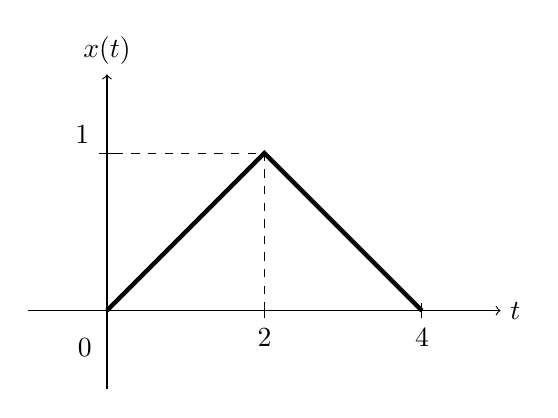
\begin{tikzpicture}
\draw[->] (-1,0) -- (5,0) node[right] {$t$};
\draw[->] (0,-1) -- (0,3) node[above] {$x(t)$};
\draw (2cm,0.1cm) -- (2cm,-0.1cm) node[below] {$2$};
\draw (4cm,0.1cm) -- (4cm,-0.1cm) node[below] {$4$};
\draw (0.1cm,2cm) -- (-0.1cm,2cm) node[above left] {$1$};
%\foreach \y in {-2,-1} {
%\draw (0.1cm,\y) -- (-0.1cm,\y) node[left] {$\y\strut$};
%}
\node[below left=0.1cm] at (-0,0) {$0\strut$};
\draw [ultra thick] (0,0) -- (2,2) -- (4,0);
\draw[dashed] (2,0) -- (2,2) -- (0,2);
\end{tikzpicture}
\end{center}





\begin{align*}
E &= \int_{-T}^{T}{x^{2}(t)dt} \\ \\
&= \int_{0}^{1}{x^{2}(t)dt} + \int_{1}^{2}{x^{2}(t)dt} \\ \\ 
&= \int_{0}^{1}{t^{2}(t)dt} + \int_{1}^{2}{(2-t)^{2}(t)dt} \\ \\ 
&= \left[ \cfrac{t^{3}}{3} \right]_{0}^{1}  + \int_{1}^{2}{ (t^{2} - 4t + 4)dt } \\ \\
&= \left[ \cfrac{t^{3}}{3} \right]_{0}^{1} +
\left[ \cfrac{t^{3}}{3} \right]_{1}^{2} - 
\left[ \cfrac{4t^{2}}{2} \right]_{1}^{2} + 
\left[ 4t \right]_{1}^{2}
\end{align*}








\section{Energy \& Power of Exponential Signal With Positive Power}



$$
x(t) = e^{at} u(t)
$$






\begin{align*}
t < 0 \to u(t) = 0  \quad \Rightarrow
\end{align*}



\begin{center}
\begin{tikzpicture}
\draw[->] (-5,0) -- (5,0) node[right] {$x$};
\draw[->] (0,-2) -- (0,3) node[above] {$y$};
\foreach \x in {-4,...,-1} {
\draw (\x,0.1cm) -- (\x,-0.1cm) node[below] {$\x\phantom{-}\strut$};
}
\foreach \x in {1,...,4} {
\draw (\x,0.1cm) -- (\x,-0.1cm) node[below] {$\x\strut$};
}
\foreach \y in {1,...,2} {
\draw (0.1cm,\y) -- (-0.1cm,\y) node[left] {$\y\strut$};
}
\foreach \y in {-1} {
\draw (0.1cm,\y) -- (-0.1cm,\y) node[left] {$\y\strut$};
}
%\node[below left=0.1cm] at (-0,0) {$0\strut$};
\draw [ultra thick] (-4,0) -- (0,0);
\begin{scope}
\clip (0,-1) rectangle (5,5);
\draw[color=red,samples=100] plot ({\x},{exp(\x)});
\end{scope}
\end{tikzpicture}
\end{center}





\begin{align*}
E &= \lim_{T\to\infty}{ \int_{-T}^{T}{x^{2}(t)dt} } \\ \\
&= \lim_{T\to\infty}{ \int_{-T}^{T}{(e^{-at} u(t))^{2}dt} } \\ \\
u(t) = 1 & \\ \\
&= \lim_{T\to\infty}{ \int_{0}^{T}{ e^{2at} dt} } \\ \\
&= \lim_{T\to\infty}{ \left[ \cfrac{ e^{2at}}{2a} \right]_{0}^{T} } \\ \\
&= \lim_{T\to\infty}{ \left[ \cfrac{ e^{2aT}}{2a} - \cfrac{e^{0}}{2a} \right] } \\ \\
&= \infty \\ \\
\Rightarrow& E = \infty
\end{align*}








\begin{align*}
P &= \lim_{T\to\infty}{ \cfrac{1}{2T} \int_{-T}^{T}{x^{2}(t)dt} } \\ \\
&= \lim_{T\to\infty}{ \cfrac{1}{2T} \int_{-T}^{T}{(e^{-at} u(t))^{2}dt} } \\ \\
u(t) = 1 & \\ \\
&= \lim_{T\to\infty}{ \cfrac{1}{2T} \int_{0}^{T}{ e^{2at} dt} } \\ \\
&= \lim_{T\to\infty}{ \cfrac{1}{2T} \left[ \cfrac{ e^{2at}}{2a} \right]_{0}^{T} } \\ \\
&= \lim_{T\to\infty}{ \cfrac{1}{2T} \left[ \cfrac{ e^{2aT}}{2a} - \cfrac{e^{0}}{2a} \right] } \\ \\
&= 0 \\ \\
\Rightarrow \quad& P = 0
\end{align*}







\section{Energy \& Power Signal Example}



Determine The Energy of The Signal given below :




\begin{center}
\begin{tikzpicture}
\draw[->] (-5,0) -- (5,0) node[right] {$t$};
\draw[->] (0,-1) -- (0,3) node[above] {$x(t)$};
\draw (-4cm,0.1cm) -- (-4cm,-0.1cm) node[below] {$-2$};
\draw (-2cm,0.1cm) -- (-2cm,-0.1cm) node[below] {$-1$};
\draw (2cm,0.1cm) -- (2cm,-0.1cm) node[below] {$1$};
\draw (4cm,0.1cm) -- (4cm,-0.1cm) node[below] {$2$};
\draw (0.1cm,2cm) -- (-0.1cm,2cm) node[above left] {$1$};
%\foreach \y in {-2,-1} {
%\draw (0.1cm,\y) -- (-0.1cm,\y) node[left] {$\y\strut$};
%}
\node[below left=0.1cm] at (-0,0) {$0\strut$};
\draw [ultra thick] (-4,0) -- (-2,2) -- (2,2) -- (4,0);
\draw[dashed] (2,0) -- (2,2) ;
\draw[dashed] (-2,0) -- (-2,2) ;
\end{tikzpicture}
\end{center}




\begin{align*}
E &= \int_{-T}^{T}{x^{2}(t)dt} \\ \\
&= \int_{-2}^{2}{x^{2}(t)dt} \\ \\
&= \int_{-2}^{-1}{(t+2)^{2}(t)dt} + \int_{-1}^{1}{(1)^{2}(t)dt} + \int_{1}^{2}{(2-t)^{2}(t)dt}
\end{align*}









\section{Energy \& Power of Ramp Signal}




\begin{align*}
R(t) = 
\begin{cases}
t & t \geq 0 \\
0 & t < 0
\end{cases}
\end{align*}







\begin{center}
\begin{tikzpicture}
\draw[->] (-5,0) -- (5,0) node[right] {$x$};
\draw[->] (0,-1) -- (0,3) node[above] {$y$};
\foreach \x in {-4,...,-1} {
\draw (\x,0.1cm) -- (\x,-0.1cm) node[below] {$\x\phantom{-}\strut$};
}
\foreach \x in {1,...,4} {
\draw (\x,0.1cm) -- (\x,-0.1cm) node[below] {$\x\strut$};
}
\foreach \y in {1,...,2} {
\draw (0.1cm,\y) -- (-0.1cm,\y) node[left] {$\y\strut$};
}
%\foreach \y in {-2,-1} {
%\draw (0.1cm,\y) -- (-0.1cm,\y) node[left] {$\y\strut$};
%}
%\node[below left=0.1cm] at (-0,0) {$0\strut$};
\draw [ultra thick] (0,0) -- (3,3);
\draw [ultra thick] (-4,0) -- (0,0);
%\draw [ultra thick, fill=black] (0,1) circle (0.1cm);
\end{tikzpicture}
\end{center}









\begin{align*}
E &= \lim_{T\to\infty}{ \int_{-T}^{T}{x^{2}(t)dt} } \\ \\
&= \lim_{T\to\infty}{ \int_{0}^{T}{x^{2}(t)dt} } \\ \\
&= \lim_{T\to\infty}{ \int_{0}^{T}{t^{2}(t)dt} } \\ \\
&= \lim_{T\to\infty}{ \left[ \cfrac{t^{3}}{3} \right]_{0}^{T} } \\ \\
&=  \lim_{T\to\infty}{ \cfrac{T^{3}}{3} } \\ \\
\Rightarrow \quad & E = \infty
\end{align*}





\begin{align*}
P &= \lim_{T\to\infty}{ \cfrac{1}{2T} \int_{-T}^{T}{x^{2}(t)dt} } \\ \\
&= \lim_{T\to\infty}{ \cfrac{1}{2T} \int_{0}^{T}{x^{2}(t)dt} } \\ \\
&= \lim_{T\to\infty}{ \cfrac{1}{2T} \int_{0}^{T}{t^{2}(t)dt} } \\ \\
&= \lim_{T\to\infty}{ \cfrac{1}{2T} \left[ \cfrac{t^{3}}{3} \right]_{0}^{T} } \\ \\
&=  \lim_{T\to\infty}{ \cfrac{1}{2T} \times \cfrac{T^{3}}{3} } \\ \\
&=  \lim_{T\to\infty}{ \cfrac{T^{2}}{6} } \\ \\
\Rightarrow \quad & P = \infty
\end{align*}





\section{Classification of Systems}


\begin{enumerate}
	\item Linear \& non-Linear Systems
	\item Time-Variant \& Time-Invariant Systems
	\item Linear Time Variant (LTV) \& Linear Time Invariant Systems (LTI)
	\item Static \& Dynamic Systems
	\item Casual \& non-Casual Systems
	\item Invertible \& non-Invertible Systems
	\item Stable \& unStable Systems
\end{enumerate}







\section{Linear \& non-Linear Systems}



A System is said to be Linear if it satisfies the superposition principle, consider a system with input $x_{1}(t)$ , $x_{2}(t)$ and output $y_{1}(t)$ , $y_{2}(t)$
for be Linear :

\begin{align*}
T[ a_{1}x_{1}(t) + a_{2}x_{2}(t) ] = a_{1}T[x_{1}(t)] + a_{2} T[x_{2}(t)]
\end{align*}




\begin{center}
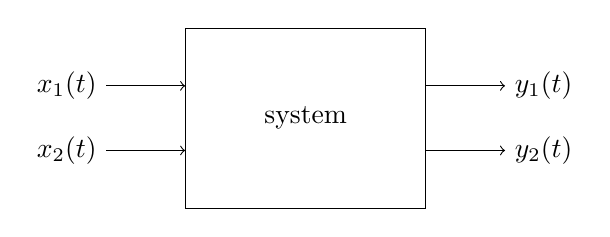
\begin{tikzpicture}
%\draw (3,1) rectangle (6,-1);
%\draw node (a) at (1,0.5) {$x_{1}(t)$};
%\draw node (a) at (1,-0.5) {$x_{2}(t)$};
%\draw node (b) at (4.5,0) {system};
\node[draw, inner sep=10mm] (b) at (4.5,0) {system};
%\draw node (c) at (8,0.5) {$y_{1}(t)$};
%\draw node (c) at (8,-0.5) {$y_{2}(t)$};
%\draw[->,->=latex,thick] (a) -- (3,0);
%\draw[->,->=latex,thick] (6,0) -- (c);
%\draw[->,->=latex,thick] (a) -- (b);
%\draw[->,->=latex,thick] (b) -- (c);
\draw[<-] (b.165) --++(180:1cm) node [left] {$x_{1}(t)$};
\draw[<-] (b.195) --++(180:1cm) node [left] {$x_{2}(t)$};
\draw[->] (b.15) --++(0:1cm) node [right] {$y_{1}(t)$};
\draw[->] (b.-15) --++(0:1cm) node [right] {$y_{2}(t)$};
\end{tikzpicture}
\end{center}


\subsubsection{example}

$$
y(t) = x^{2}(t)
$$


\begin{align*}
T[x_{1}(t)] &=  x_{1}^{2}(t) \Rightarrow a_{1} T[x_{1}(t)] = a_{1} x_{1}^{2}(t)  \\ 
T[x_{2}(t)] &=  x_{2}^{2}(t) \Rightarrow a_{2} T[x_{2}(t)] = a_{2} x_{2}^{2}(t)
\end{align*}






\begin{align*}
T[ a_{1}x_{1}(t) + a_{2}x_{2}(t) ] = [ a_{1}x_{1}(t) + a_{2}x_{2}(t) ]^{2} 
\end{align*}






\begin{align*}
&\Rightarrow T[ a_{1}x_{1}(t) + a_{2}x_{2}(t) ] \neq a_{1} T[x_{1}(t)] + a_{2} T[x_{2}(t)] \\ \\
&\Rightarrow \text{The System is non-Linear}
\end{align*}










\newpage

\subsubsection{example}




$$
y(t) = x(t)
$$


\begin{align*}
T[x_{1}(t)] &=  x_{1}(t) \Rightarrow a_{1} T[x_{1}(t)] = a_{1} x_{1}(t)  \\ 
T[x_{2}(t)] &=  x_{2}(t) \Rightarrow a_{2} T[x_{2}(t)] = a_{2} x_{2}(t)
\end{align*}





\begin{align*}
T[ a_{1}x_{1}(t) + a_{2}x_{2}(t) ] = [ a_{1}x_{1}(t) + a_{2}x_{2}(t) ]
\end{align*}





\begin{align*}
&\Rightarrow T[ a_{1}x_{1}(t) + a_{2}x_{2}(t) ] = a_{1} T[x_{1}(t)] + a_{2} T[x_{2}(t)] \\ \\
&\Rightarrow \text{The System is Linear}
\end{align*}











\section{Time-Variant \& Time-Invariant Systems}



A System is said to be time variant if its input, output characteristics change with time , otherwise said to be time invariant .

The condition for time invariant is 
$$
y(n,k) = y(n-k)
$$
where
$$
y(n,k) = T[x(n-k)]
$$







\subsubsection{example}



$$
y(n) = x(n) + x(n-2)
$$





\begin{align*}
y(n,k) &= T[x(n-k)] \\ 
&= x(n-k) + x(n-2-k)
\end{align*}




\begin{align*}
y(n-k) &= x(n-k) + x(n-k-2) \\ 
&\Rightarrow y(n,k) = y(n-k) \\
&\Rightarrow \text{System is Time-Invariant}
\end{align*}







\subsubsection{example}



$$
y(n) = x(n) + nx(n-3)
$$




\begin{align*}
y(n,k) &= T[x(n-k)] \\ 
&= x(n-k) + n x(n-k-3)
\end{align*}




\begin{align*}
y(n-k) &= x(n-k) +  (n-k) x(n-k-3) \\ 
&\Rightarrow y(n,k) \neq y(n-k) \\
&\Rightarrow \text{System is Time Variant}
\end{align*}







\section{Linear Time Variant (LTV) \& Linear Time Invariant Systems (LTI)}



A System is said to be LTV when it satisfies both Linearity \& Time Variant .

A System is said to be LTI when it satisfies both Linearity \& Time InVariant .






\subsubsection{example}

check for linearity

$$
y(n) = n x^{2}(n)
$$




\begin{align*}
y_{1}(t) = T[x_{1}(t)] &=  n x_{1}^{2}(t) \Rightarrow a_{1} T[x_{1}(t)] = a_{1} n x_{1}^{2}(t)  \\ 
y_{2}(t) = T[x_{2}(t)] &=  n x_{2}^{2}(t) \Rightarrow a_{2} T[x_{2}(t)] = a_{2} n x_{2}^{2}(t)
\end{align*}




\begin{align*}
T[ a_{1}x_{1}(t) + a_{2}x_{2}(t) ] = n [ a_{1}x_{1}(t) + a_{2}x_{2}(t) ]^{2} 
\end{align*}

\begin{align*}
&\Rightarrow T[ a_{1}x_{1}(t) + a_{2}x_{2}(t) ] \neq a_{1} T[x_{1}(t)] + a_{2} T[x_{2}(t)] \\ \\
&\Rightarrow \text{The System is non-Linear}
\end{align*}





check for time variant or invariant .


$$
y(n) = n x^{2}(n)
$$




\begin{align*}
y(n,k) &= T[x(n-k)] \\ 
&=  n x^{2}(n-k)
\end{align*}




\begin{align*}
y(n-k) &=  (n-k) x^{2}(n-k) \\ 
&\Rightarrow y(n,k) \neq y(n-k) \\
&\Rightarrow \text{System is Time Variant}
\end{align*}






\subsubsection{example}



$$
y(n) = x(n-2)
$$


check for linearity

\begin{align*}
y_{1}(t) = T[x_{1}(t)] &=  x_{1}(t-2) \Rightarrow a_{1} T[x_{1}(t)] = a_{1} x_{1}(t-2)  \\ 
y_{2}(t) = T[x_{2}(t)] &=  x_{2}(t-2) \Rightarrow a_{2} T[x_{2}(t)] = a_{2} x_{2}(t-2)
\end{align*}




\begin{align*}
T[ a_{1}x_{1}(t) + a_{2}x_{2}(t) ] &= a_{1}x_{1}(t-2) + a_{2}x_{2}(t-2) \\ \\ 
\Rightarrow T[ a_{1}x_{1}(t) + a_{2}x_{2}(t) ] &= a_{1}T[x_{1}(t)] + a_{2}T[x_{2}(t)] \\ \\
&\Rightarrow \text{The System is Linear}
\end{align*}






check for time variant or invariant .




$$
y(n) = x(n-2)
$$



\begin{align*}
y(n,k) &= T[x(n-k)] \\ 
&=  x(n-k-2)
\end{align*}




\begin{align*}
y(n-k) &= x(n-k-2) \\ 
&\Rightarrow y(n,k) = y(n-k) \\
&\Rightarrow \text{System is Time Invariant}
\end{align*}








\section{Static \& Dynamic Systems}



Static System is memoryless system where as Dynamic System is with memory System .



e.g : 


\begin{align*}
y(n) &= x(n) \\ 
y(0) &= x(0) \to \text{Static}
\end{align*}


e.g : 

\begin{align*}
y(t) &= 2 x^{2}(t) \\ 
y(-2) &= 2 x^{2}(-2) \to \text{Static}
\end{align*}




e.g : 

\begin{align*}
y(n) &= x(n) + x(n-1) \\ 
y(1) &= x(1) + x(1-1) \\ 
&= x(1) + x(0) \to \text{Dynamic}
\end{align*}



e.g : 

\begin{align*}
y(t) &= x(t) + x(t+3) \\ 
y(-1) &= x(-1) + x(-1+3) \\ 
&= x(-1) + x(2) \to \text{Dynamic}
\end{align*}






\section{Casual \& non-Casual Systems}


A System is said to be casual if its response is dependent upon present \& past inputs \& doesn't depends upon future input .


for a non-casual System The output depends upon future input too .


\noindent 
e.g : 


\begin{align*}
y(n) &= x(n) + \cfrac{1}{x(n-1)} \\
y(1) &= x(1) + \cfrac{1}{x(1-1)} \\
y(1) &= x(1) + \cfrac{1}{x(0)} \Rightarrow \text{Casual}
\end{align*}


\noindent 
e.g : 

\begin{align*}
y(t) &= 2x(t) + \cfrac{1}{x^{2}(t)} \\
y(0) &= 2x(0) + \cfrac{1}{x^{2}(0)} \\
&= x(1) + \cfrac{1}{x(0)} \Rightarrow \text{Casual}
\end{align*}



\noindent 
e.g : 


\begin{align*}
y(n) &= x(n) + \cfrac{1}{2x(n+1)} \\
y(0) &= x(0) + \cfrac{1}{2x(1)} \\
&= x(1) + \cfrac{1}{x(0)} \Rightarrow \text{non-Casual}
\end{align*}


\noindent 
e.g : 


\begin{align*}
y(t) &= x(t) + x(t-1) + \cfrac{1}{x(t+1)} \\
y(0) &= x(0) + x(0-1) + \cfrac{1}{x(0+1)} \\
y(0) &= x(0) + x(-1) + \cfrac{1}{x(1)} \Rightarrow \text{non-Casual}
\end{align*}



\begin{tcolorbox}
All Static Systems Are Casual but not Vice Versa
\end{tcolorbox}

\begin{tcolorbox}
All non-Casual Systems Are Dynamic but not Vice Versa
\end{tcolorbox}



\section{Invertible \& non-Invertible Systems}


A System is said to be Invertible if the input of the system appears at the output 


\begin{center}
\begin{tikzpicture}
%\draw (3,1) rectangle (6,-1);
\draw node (a) at (1,0) {$x(t)$};
%\draw node (b) at (4.5,0) {system};
\node[draw, inner sep=8mm] (b1) at (4.5,0) {$h_{1}(t)$};
\node[draw, inner sep=8mm] (b2) at (8.5,0) {$h_{2}(t)$};
\draw node (c) at (12,0) {$y(t) = x(t)$};
%\draw[->,->=latex,thick] (a) -- (3,0);
%\draw[->,->=latex,thick] (6,0) -- (c);
\draw[->,->=stealth,thick] (a) -- (b1);
\draw[->,->=stealth,thick] (b1) -- (b2);
\draw[->,->=stealth,thick] (b2) -- (c);
\end{tikzpicture}
\end{center}


if $y(t) \neq x(t)$ then the system is non-invertible





\section{Stable \& unStable Systems}


A System is said to be stable when it produces bounded output for a bounded input .


e.g :

\begin{align*}
y(n) = x^{2}(n) \to \text{stable}
\end{align*}

e.g : 


\begin{align*}
y(t) = \int{x(t)dt} \to \text{unstable}
\end{align*}




\end{document}